\documentclass[Methods]{subfiles}
\begin{document}
\section{Methods}
\label{sec:Methods}

In order to find the overhead Naxsi has when it is actively used as a \ac{WAF}, it is important to create a baseline reference to compare the results to. First, the performance is measured when there is processing of any application data taken place. This is done by returning HTTP 200 OK message to the client. This way there is a minimal overhead and this makes it possible to isolate Naxsi as much as possible. Second, the performance is measure with a default Wordpress installation. In both cases, the performance is measured first with Naxsi being disabled and later with Naxsi enabled.

Before both scenarios are discussed in more depth, it is important to understand how the basic configuration is setup. A configuration for standard web hosting that is seen quite often, is to separate the web hosting services on a functional basis. First, there is the web server, this the front-end from a client's perspective. Second, there is application layer. The application layer takes care of most of the processing power that is needed to process all the data. Third, there is the data layer, which is often a database server. It is not necessary to separate these layers over different servers. Depending on the requirements, it is possible to host all services on one server. In order to do a performance measurement on one of these services, it is important that not all services run on the same server. Therefore, in this setup, every layer has a dedicated server. In the next section the setup is discussed more in depth.

\subsection{Experimental setup}

Figure \ref{fig:Experimental setup} shows the setup that is used during the experiments. Table \ref{tab:Experimental infrastructure} gives a short description of each server and the service(s) that run(s) on it. Server01 is the front-end server, but it will also act as a software router for basic communication with the servers behind it. Server02 processes all the application data, which for a large part consists of the processing of PHP code. The hardware specification and the software that is used, can be found in appendix \ref{sec:Experimental setup}.

\begin{figure}[h]
\caption{Experimental setup}
\centering
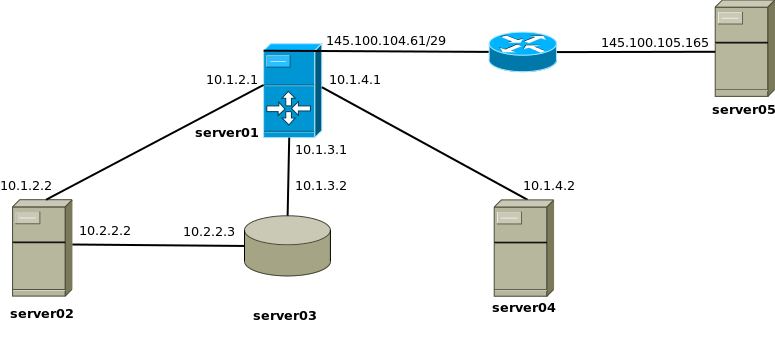
\includegraphics[scale=0.4] {images/infrastructure.png}
\label{fig:Experimental setup}
\end{figure}

\begin{table}[h]
\caption{Experimental infrstructure}
\begin{tabular}{|p{2,5cm}|p{3,5cm}|p{5cm}|}
\hline
\textbf{Hostname} & \textbf{Service} & \textbf{Short description} \\ \hline
server01 & Nginx + Naxsi & Front-end server and router \\ \hline
server02 & Nginx + Fastcgi & Application layer \\ \hline
server03 & MySQL & Data layer \\ \hline
server04 & Benchmark tools & Performance measurement \\ \hline
server05 & Collectd & Performance data collector \\ \hline
\end{tabular}
\label{tab:Experimental infrastructure}
\end{table}

\subsection{Performance measurement tools}
A variety of performance measurement tools (also called benchmarking tools) exist. However not all of them are suited to perform tests in this specific experimental setup while also not influencing the measurement. This section discusses a selection of tools. The sections of those that have in fact been used, specify the way they were set up.

\subsubsection{Apache Benchmark}
\emph{Apache Benchmark} is an open source web server benchmarking tool developed by Apache initially to test Apache web server installations.\footnote{\url{http://httpd.apache.org/docs/2.2/programs/ab.html}} However, it is not limited to Apache web servers, as it simulates regular HTTP requests.\\
During the execution of the performance tests, \emph{Apache Benchmark} is used when the number requests per second exceed the number of concurrent connections that are realistically possible. To be able to stepwise increase the number or URL parameters, as well as to calculate the avarage of repeated tests, a perl script is written to automate these operations~\footnote{\url{https://github.com/lutzengels/naxsiperftest/blob/master/tools/bench.pl}}.  These experiments are explained later in this section.


\subsubsection{Httperf}
%\emph{Httperf} is a web server performance measurement tool developed by David Mosberger~\cite{mosberger1998httperf} at Hewlet-Packard Research Labs~\cite{httperf}. It supports both HTTP/1.1 and SSL and aims to be robust enough to generate server overload. \emph{Autobench}~\cite{autobench2013} is a Perl script that wraps around \emph{Httperf}. It aims at automating the benchmarking process and offers extensive options, amongst which the ability to stepwise increase concurrent connections or the number of requests per second. 

In the course of this project, \emph{Autobench} is used to confirm and visualize the threshold of the number of concurrent connections that Naxsi can handle (as described in section~\ref{sec:Baseline performance measurement}). The automation of incrementing the URL parameters is done by wrapping a script~\footnote{\url{https://github.com/lutzengels/naxsiperftest/blob/master/tools/measure_naxsi_with_param_increments.pl}} around Autobench.


\subsubsection{Autobench}
\emph{Autobench} is a Perl script that instruments \emph{httperf} to benchmark web servers. It offers extensive options, amongst which the ability to stepwise increase concurrent connections or the number of request. This results in graphs that visualize bottlenecks/tipping points.


\subsubsection{Collectd}
Collectd is a daemon for unix-based operating systems that gathers performance statistics. It has a modular design, meaning that the different kind of statistics (like e.g. cpu-load or network-usage) are en- or disabled by toggling the respective plugins and thereby minimizing resource usage. Furthermore it only handles the data collection and storage hereof, leaving out logic to create graphs, whilst storing data in \ac{RRD} files. Programs like RRDtool in turn can easily create graphs from the RRD-files. It is written in the fast and low impact programming language C~\cite{prechelt2000empirical} and designed to be run on e.g. embedded devices.
As to influence the experimental setup as little as possible Collectd appeared to be the right choice.

Collectd is configured on all servers of the experimental setup. \emph{server01} to \emph{server04} are configured as clients, collecting their own local performance data. \emph{server05} also collects its own local performance data, but also receives those from the clients. Making use of the \emph{collection3} web-based front-end RRDtool is utilized to graph the collected data.
\\
For detailed configuration please refer to Appendix~\ref{sec:Configuration}.


\subsection{Performance measurements}
The performance measurement is done in two phases. The first phase is to measure the baseline performance of the Nginx webserver without Naxsi compiled into it. These measurements are needed to later see the overhead when Naxsi is enabled, as is done in the second phase. In both phases the performance is measured with a Wordpress website on a back-end server and when the Nginx server simply returns an \verb+HTTP 200 OK+ reponse. Details of how the Nginx server is compiled with Naxsi or without can be found in \ref{{sec:server01_configuration}}.

The Wordpress website is introduced in the measurement to see the effects of a more realistic scenario. Based on the \ac{CMS} popularity measurements of March 1st by w3techs \footnote{\url{http://w3techs.com/technologies/overview/content_management/all}}, Wordpress is chosen as the web application. According to their survey, 17,4 \% of all web servers run Wordpress and it holds 54,6 \% of the CMS market share. Wordpress has, by far, the greatests market share and is therefore a popular target for cyber criminals. Naxsi, of course, should block most of these cyber attacks.

\subsubsection{Wordpress}
For the performance measurement when a Wordpress site is active, httperf has proven to be a reliable tool. By measuring the response time of each request and by monitoring the resources on the front-end server, it shows the impact of simply hosting a Wordpress website. This is repeated for both the baseline measurement as for when Naxsi is actively protecting the website.

\subsubsection{HTTP 200 OK}
In order to measure the performance when Nginx replies with \verb+HTTP 200 OK+ messages, httperf is not suitable anymore. The number of requests per second exceed the number of concurrents that are realisticly possible. Instead, the Apache benchmark tools are used. However, the number of requests per second are far greater than that of when a Wordpress website is hosted. Because of the high number of concurrent connections, Apache benchmark shows some discrepencies that need to be taken into consideration. Each individual Apache benchmark command is repeated 5 times, also revered to as a round. A set of rounds is called a step. Of each step, the lowest, highest and average values are graphed to show the discrepancies.

In order to measure the impact Naxsi has on processing the content of the request, we focus on the number of URL parameters. Naxsi has to process each parameter and see if it is allowed. Based on the optimal concurrent connections measured during the baseline measurement, the next thing to be looked at is the number of URL parameters.

\begin{verbatim}
http://200_with_naxsi.test.nl/
http://200_with_naxsi.test.nl/?foo1=bar1
http://200_with_naxsi.test.nl/?foo1=bar1&foo2=bar2
...
\end{verbatim}
\end{document}

